\chapter{CƠ SỞ LÝ THUYẾT VÀ CÁC CÔNG TRÌNH LIÊN QUAN}
\label{chap:lythuyet}

Chương này trình bày cơ sở lý thuyết về hệ thống gợi ý, các mô hình được sử dụng trong đề tài và các công trình liên quan. Các công trình được dẫn là cơ sở về phương pháp (định nghĩa mô hình, cách huấn luyện, cách đánh giá); thực nghiệm trong các công trình đó dùng dữ liệu và giao thức khác nên số liệu của chúng không được dùng làm chuẩn để so sánh với kết quả của đề tài. Trong chương này, \emph{User} (người dùng) và \emph{Item} (sản phẩm) được dùng như thuật ngữ kỹ thuật theo cách gọi phổ biến trong tài liệu về hệ gợi ý.

\section{Tổng quan về hệ thống gợi ý (Recommendation System)}
\label{sec:tongquan_rs}

\subsection{Lọc nội dung, lọc cộng tác và lọc lai: lựa chọn của đề tài}
\label{subsec:khainiem_rs}

Một hệ thống gợi ý có ba hướng tiếp cận chính. \textbf{Lọc dựa trên nội dung} (Content-Based) gợi ý những sản phẩm có đặc tính giống các sản phẩm User đã thích, dựa trên mô tả sản phẩm và hồ sơ sở thích của User \parencite{lops2011content, schafer2001commerce}. \textbf{Lọc cộng tác} (Collaborative Filtering -- CF) khai thác lịch sử tương tác chung giữa nhiều User và Item: những User từng mua giống nhau có khả năng sẽ mua giống nhau \parencite{koren2009matrix, sarwar2001item}; CF chỉ cần ma trận tương tác User--Item, không đòi hỏi đặc trưng mô tả đối tượng \parencite{su2009survey}. \textbf{Lọc lai} (Hybrid) kết hợp nhiều kỹ thuật -- thường gặp nhất là kết hợp nội dung với cộng tác -- để bù hạn chế của từng kỹ thuật \parencite{burke2002hybrid, cheng2016wide, guo2017deepfm}.

Lựa chọn của đề tài được quyết định bởi \emph{đặc điểm của dữ liệu}. Bộ dữ liệu H\&M (mục~\ref{subsec:hm_description}) có lịch sử giao dịch đủ dài để CF học được sở thích của khách mua thường xuyên, nhưng danh mục thời trang thay đổi rất nhanh: một phần đáng kể sản phẩm khách mua trong vài tuần tới là sản phẩm chưa từng được bán (mục~\ref{subsec:split_sampling}). CF thuần dựa trên ID không có thông tin gì về những sản phẩm này, trong khi bộ dữ liệu lại có sẵn thuộc tính, mô tả văn bản của sản phẩm, thông tin khách hàng và doanh số theo thời gian. Vì vậy đề tài chọn hướng \textbf{lai}: lõi của mô hình là lọc cộng tác dựa trên mô hình -- nhân tử hóa ma trận kết hợp mạng nơ-ron sâu (mục~\ref{sec:cf_mf}, \ref{sec:ncf_architecture}) -- được bổ sung đặc trưng nội dung và ngữ cảnh (mục~\ref{subsec:deep_ctr}). Các mô hình chỉ dùng ID và một mô hình gợi ý theo nội dung thuần được giữ làm đối chứng, để đo riêng đóng góp của từng nguồn thông tin.

\subsection{Lọc cộng tác dựa trên bộ nhớ (Memory-based) và dựa trên mô hình (Model-based)}
\label{subsec:memory_model_based}

Xét theo cách khai thác dữ liệu tương tác, các phương pháp Lọc cộng tác được chia thành hai nhánh chính, đặt nền móng lý thuyết cho toàn bộ hướng tiếp cận Model-based mà đề tài lựa chọn.

\textbf{Lọc cộng tác dựa trên bộ nhớ (Memory-based CF)} tính toán trực tiếp độ tương đồng giữa các User hoặc Item từ ma trận tương tác thô, không qua bước học tham số trung gian, theo nguyên lý khởi nguồn của hệ thống GroupLens \parencite{resnick1994grouplens}. Với \textbf{Item-based CF} \parencite{sarwar2001item} -- kỹ thuật được Amazon triển khai thành công ở quy mô công nghiệp \parencite{linden2003amazon} -- độ tương đồng cosine giữa hai sản phẩm $i, j$ được tính theo vector cột tương tác của chúng:
\begin{equation}
    \text{sim}(i, j) = \cos(\vec{i}, \vec{j}) = \frac{\vec{i} \cdot \vec{j}}{\lVert \vec{i} \rVert \, \lVert \vec{j} \rVert}
    \label{eq:cosine_sim}
\end{equation}
Với phản hồi ẩn nhị phân, điểm của sản phẩm $i$ cho User $u$ là tổng độ tương đồng giữa $i$ và những sản phẩm $u$ đã mua, chỉ xét $k$ láng giềng gần nhất $\mathcal{N}_k(i)$ của $i$ (ItemKNN):
\begin{equation}
    \hat{y}_{ui} = \sum_{j \in \mathcal{N}_k(i) \cap \mathcal{I}_u} \text{sim}(i, j)
    \label{eq:itemcf_predict}
\end{equation}
Đối xứng với cách trên, \textbf{User-based CF} (UserKNN) tìm $k$ User có lịch sử mua giống $u$ nhất, $\mathcal{N}_k(u)$ -- chính là ``Top-$K$ người dùng tương đồng'' của $u$ -- rồi tính điểm mỗi sản phẩm bằng tổng độ tương đồng của những láng giềng đã mua sản phẩm đó:
\begin{equation}
    \hat{y}_{ui} = \sum_{v \in \mathcal{N}_k(u)} \text{sim}(u, v)\, y_{vi}
    \label{eq:usercf_predict}
\end{equation}
Trong cài đặt của đề tài, độ tương đồng cosine được tính trên vector mua nhị phân, có thêm hệ số co (shrink) $\lambda$ ở mẫu số để giảm trọng số của những cặp chỉ có rất ít tương tác chung: $\text{sim}(a, b) = |\mathcal{I}_a \cap \mathcal{I}_b| / (\sqrt{|\mathcal{I}_a|\,|\mathcal{I}_b|} + \lambda)$, với $\mathcal{I}_a$ là tập sản phẩm $a$ đã mua (hoặc tập User đã mua sản phẩm $a$). Mỗi hàng của ma trận tương đồng chỉ giữ $k$ láng giềng và được lưu dưới dạng ma trận thưa, nên chạy được với khoảng 10.000 sản phẩm; $k$ và $\lambda$ được chọn trên tập xác thực, và hai mô hình là baseline của đề tài (mục~\ref{sec:baselines}). Ưu điểm của nhánh này là đơn giản, không cần huấn luyện và dễ diễn giải -- có thể chỉ ra cụ thể những User hoặc sản phẩm nào dẫn tới một gợi ý; nhược điểm là ma trận tương đồng đầy đủ tăng bậc hai theo số thực thể ($O(N^2)$) và chất lượng suy giảm khi ma trận tương tác quá thưa.

\textbf{Lọc cộng tác dựa trên mô hình (Model-based CF)} không tính tương đồng trực tiếp mà học một hàm tham số hóa (Nhân tử hóa ma trận, mạng nơ-ron) để nén thông tin tương tác thành các vector biểu diễn ẩn có số chiều thấp, cho phép tổng quát hóa tốt hơn trên dữ liệu thưa và mở rộng quy mô tuyến tính theo số lượng tương tác thay vì bậc hai theo số Item \parencite{koren2009matrix, su2009survey}. Toàn bộ các mô hình MF, GMF, MLP và NeuMF trình bày từ mục~\ref{sec:cf_mf} trở đi thuộc nhánh Model-based, là hướng tiếp cận chính của đề tài.

\subsection{Vì sao bài toán buộc phải dùng phản hồi ẩn (Implicit Feedback)}
\label{subsec:feedback_types}

Về nguyên tắc, phản hồi của User có thể là phản hồi hiện (Explicit) -- điểm số đánh giá trực tiếp như rating 1--5 sao -- hoặc phản hồi ẩn (Implicit) -- suy ra gián tiếp từ hành vi như lịch sử mua hàng, lượt click \parencite{he2017ncf, rendle2009bpr}. Điểm cần nói rõ ở đây không phải là định nghĩa chung của hai khái niệm này, mà là một ràng buộc thực tế: tệp giao dịch H\&M không có bất kỳ cột đánh giá (rating) nào -- chỉ có bản ghi giao dịch đã xảy ra. Điều này loại bỏ hoàn toàn khả năng dùng Explicit Feedback, và buộc toàn bộ đề tài phải xây dựng tín hiệu tương tác dưới dạng nhị phân từ chính sự kiện mua hàng:
\begin{equation}
    y_{ui} = \begin{cases}
        1, & \text{nếu tồn tại giao dịch giữa User } u \text{ và Item } i \text{ trong dữ liệu} \\
        0, & \text{ngược lại}
    \end{cases}
    \label{eq:implicit_binary}
\end{equation}
Hệ quả trực tiếp của cách xây dựng nhãn này -- $y_{ui}=1$ chỉ xác nhận \emph{đã mua}, không xác nhận \emph{hài lòng}, và $y_{ui}=0$ có thể là ``chưa từng biết đến sản phẩm'' chứ không hẳn ``không thích'' \parencite{he2017ncf} -- là lý do trực tiếp khiến kỹ thuật lấy mẫu âm (Negative Sampling, mục~\ref{subsec:dynamic_sampling}) phải được thiết kế cẩn thận thay vì coi mọi cặp chưa tương tác là nhãn âm chắc chắn đúng.

\subsection{Độ thưa dữ liệu và khởi đầu lạnh: hai giới hạn định hình thiết kế của đề tài}
\label{subsec:thachthuc_sparsity}

Hai thách thức kinh điển của Collaborative Filtering trực tiếp định hình thiết kế mô hình và phạm vi thực nghiệm của đề tài (mục~\ref{subsec:phamvi}):
\begin{itemize}
    \item \textbf{Độ thưa dữ liệu (Data Sparsity):} Số cặp User--Item thực sự có tương tác chỉ chiếm một phần rất nhỏ trong toàn bộ ma trận $M \times N$ \parencite{koren2009matrix}. Trên dữ liệu của đề tài (Bảng~\ref{tab:kcore_hm}, Bảng~\ref{tab:kcore_hm_full}), ngay cả sau khi lọc $k$-core, mật độ chỉ khoảng 0,28\% trên mẫu thực nghiệm ($k=10$), và chỉ 0,03\% trên toàn bộ 889.062 người dùng ở quy mô đầy đủ ($k=5$).
    \item \textbf{Khởi đầu lạnh (Cold-Start):} xảy ra khi một User hoặc Item chưa có lịch sử tương tác, khiến mô hình CF không có dữ liệu để học vector biểu diễn cho đối tượng đó \parencite{schein2002coldstart}. Đề tài phân biệt hai trường hợp. \emph{Khởi đầu lạnh của người dùng} nằm ngoài phạm vi: mọi khách được đánh giá đều có lịch sử mua trước mốc dự đoán (sau lọc $k$-core, mục~\ref{subsec:interaction_matrix}). \emph{Khởi đầu lạnh của sản phẩm} thì không thể tránh với dữ liệu thời trang -- sản phẩm mới ra mắt liên tục -- nên được đưa vào phạm vi đánh giá: sản phẩm chưa từng bán trước mốc dự đoán vẫn nằm trong tập ứng viên (mục~\ref{subsec:split_sampling}), và mô hình đề tài chấm điểm chúng bằng đặc trưng nội dung (mục~\ref{subsec:deep_ctr}, \ref{sec:model_design}).
\end{itemize}

\section{Cơ sở lý thuyết về Lọc cộng tác và Nhân tử hóa ma trận}
\label{sec:cf_mf}

\subsection{Mô hình Nhân tử hóa ma trận (Matrix Factorization -- MF)}
\label{subsec:mf_model}

Nhân tử hóa ma trận (MF) chiếu cả User và Item vào một không gian đặc trưng ẩn chung có số chiều $d \ll \min(M, N)$ \parencite{koren2009matrix}. Mỗi User $u$ được biểu diễn bởi vector $p_u \in \mathbb{R}^d$ và mỗi Item $i$ bởi vector $q_i \in \mathbb{R}^d$. Mức độ tương tác dự đoán $\hat{y}_{ui}$ được tính bằng tích vô hướng:
\begin{equation}
    \hat{y}_{ui} = p_u^T q_i = \sum_{f=1}^{d} p_{uf} q_{if}
    \label{eq:mf_dot}
\end{equation}
Các kỹ thuật MF khác nhau ở cách học hai ma trận nhân tử $P$ và $Q$. Phân rã giá trị kỳ dị (Singular Value Decomposition -- SVD) cổ điển phân rã một ma trận \emph{đầy đủ}, nên không áp dụng trực tiếp được cho ma trận tương tác cực thưa, nơi phần lớn ô chưa được quan sát; các biến thể dùng trong hệ gợi ý thay vào đó tối ưu sai số trên các ô đã biết kèm điều chuẩn \parencite{koren2009matrix}. Với phản hồi ẩn, Bình phương tối thiểu luân phiên (Alternating Least Squares -- ALS) dạng iALS \parencite{hu2008implicit} coi mọi ô là quan sát với độ tin cậy khác nhau và luân phiên giải bài toán bình phương tối thiểu cho $P$ khi cố định $Q$ rồi ngược lại; còn BPR (mục~\ref{subsec:bpr}) tối ưu trực tiếp thứ hạng theo cặp. Đề tài dùng BPR-MF làm baseline MF chính; iALS \parencite{rendle2022ials} chỉ được thử trong giai đoạn phát triển (mục~\ref{sec:v1_history}).

\subsection{Hạn chế của tích vô hướng trong mô hình hóa tương tác}
\label{subsec:mf_limitations}

Tích vô hướng kết hợp các chiều đặc trưng ẩn độc lập theo dạng tuyến tính. \textcite{he2017ncf} lập luận rằng vì vậy phép toán này không học được các tương tác phức tạp, phi tuyến giữa các chiều đặc trưng của User và Item, và không đủ linh hoạt để biểu diễn chính xác quan hệ tương đồng giữa các User trong không gian ẩn. Lập luận này là động cơ lý thuyết của kiến trúc NCF (mục~\ref{sec:ncf_architecture}); việc bổ sung thành phần phi tuyến có thực sự cải thiện chất lượng gợi ý hay không phụ thuộc vào dữ liệu, và được đề tài kiểm tra bằng thực nghiệm trên dữ liệu H\&M (Chương~\ref{chap:thucnghiem}).

\subsection{Tối ưu hóa xếp hạng theo cặp: Bayesian Personalized Ranking (BPR)}
\label{subsec:bpr}

Khác với cách tiếp cận Pointwise (dự đoán độc lập từng điểm $\hat{y}_{ui}$ rồi so khớp với nhãn nhị phân như MF/GMF/MLP), Bayesian Personalized Ranking (BPR) \parencite{rendle2009bpr} tối ưu hóa trực tiếp \emph{thứ hạng tương đối} theo cặp (Pairwise Ranking), xuất phát từ giả định người dùng luôn ưa thích sản phẩm đã tương tác $i$ hơn sản phẩm chưa tương tác $j$. Với mỗi bộ ba $(u, i, j)$ trong đó $i \in \mathcal{I}_u$ và $j \notin \mathcal{I}_u$, hàm mất mát BPR cực đại hóa xác suất hậu nghiệm dưới dạng:
\begin{equation}
    \mathcal{L}_{BPR} = -\sum_{(u,i,j) \in \mathcal{D}_S} \ln \sigma\left(\hat{y}_{ui} - \hat{y}_{uj}\right) + \lambda_\Theta \lVert \Theta \rVert^2
    \label{eq:bpr_loss}
\end{equation}
trong đó $\hat{y}_{ui}, \hat{y}_{uj}$ được tính theo Công thức~\eqref{eq:mf_dot} khi kết hợp với MF (tạo thành baseline BPR-MF dùng trong Chương~\ref{chap:thucnghiem}), và $\mathcal{D}_S$ là tập các bộ ba lấy mẫu. So với hàm tổn thất Binary Cross-Entropy theo hướng Pointwise được NeuMF sử dụng (Công thức~\eqref{eq:bce_loss}), mục tiêu Pairwise của BPR bám sát hơn với bản chất bài toán xếp hạng Top-K nhưng không tận dụng được các tầng phi tuyến sâu như kiến trúc NCF.

\section{Kiến trúc Mạng khuyến nghị thần kinh (Neural Collaborative Filtering -- NCF)}
\label{sec:ncf_architecture}

\subsection{Generalized Matrix Factorization (GMF)}
\label{subsec:gmf}

Generalized Matrix Factorization (GMF) là sự mở rộng của MF dưới dạng biểu diễn mạng nơ-ron \parencite{he2017ncf}, thực hiện phép nhân Element-wise (Hadamard product $\odot$) giữa vector Embedding của User $p_u^G$ và Item $q_i^G$:
\begin{equation}
    \phi^{GMF} = p_u^G \odot q_i^G
    \label{eq:gmf_hadamard}
\end{equation}
\begin{equation}
    \hat{y}_{ui}^{GMF} = \sigma \left( h^T \phi^{GMF} \right) = \sigma \left( h^T (p_u^G \odot q_i^G) \right)
    \label{eq:gmf_predict}
\end{equation}
trong đó $\odot$ là phép nhân từng phần tử, $h$ là vector trọng số lớp đầu ra, và $\sigma(x) = \frac{1}{1 + e^{-x}}$ là hàm kích hoạt Sigmoid.

\subsection{Multi-Layer Perceptron (MLP)}
\label{subsec:mlp}

Nhánh Multi-Layer Perceptron (MLP) nối vector Embedding $p_u^M$ và $q_i^M$ (Concatenation) làm đầu vào cho chuỗi các lớp mạng liên tiếp \parencite{he2017ncf}:
\begin{equation}
    z_1 = \phi_1^{MLP} = \begin{bmatrix} p_u^M \\ q_i^M \end{bmatrix}
    \label{eq:mlp_concat}
\end{equation}
\begin{equation}
    \phi_L^{MLP} = a_L \left( W_L^T \phi_{L-1}^{MLP} + b_L \right)
    \label{eq:mlp_layerL}
\end{equation}
trong đó $W_L, b_L, a_L$ lần lượt là trọng số, độ lệch (bias) và hàm kích hoạt phi tuyến (như ReLU) tại lớp thứ $L$. Cấu trúc này giúp mô hình học các tương tác phi tuyến tính phức tạp giữa đặc trưng của User và Item.

\subsection{Kiến trúc mô hình lai NeuMF}
\label{subsec:neumf_arch}

Mô hình lai NeuMF kết hợp song song hai luồng biểu diễn tuyến tính (GMF) và phi tuyến (MLP) trước lớp dự đoán cuối cùng \parencite{he2017ncf}:
\begin{equation}
    \phi^{NeuMF} = \begin{bmatrix} \phi^{GMF} \\ \phi_L^{MLP} \end{bmatrix} = \begin{bmatrix} p_u^G \odot q_i^G \\ \phi_L^{MLP} \end{bmatrix}
    \label{eq:neumf_concat}
\end{equation}
\begin{equation}
    \hat{y}_{ui} = \sigma \left( h^T \begin{bmatrix} p_u^G \odot q_i^G \\ \phi_L^{MLP} \end{bmatrix} \right)
    \label{eq:neumf_prediction}
\end{equation}
Chữ ``lai'' trong tên đề tài trước hết chỉ việc kết hợp hai cách mô hình hóa tương tác -- nhân tử hóa ma trận (tuyến tính) và mạng nơ-ron sâu (phi tuyến) -- trong cùng một mô hình, đúng như NeuMF được \textcite{he2017ncf} xây dựng bằng cách hợp nhất GMF với MLP. Theo phân loại cách hợp nhất ở mục~\ref{subsec:early_late_fusion}, NeuMF là một mô hình Early Fusion ở mức biểu diễn. Mô hình đề tài NeuMF-F (mục~\ref{sec:model_design}) giữ đúng cấu trúc này và bổ sung đặc trưng nội dung của sản phẩm, thông tin khách hàng và thời gian vào vector của cả hai nhánh, nên còn là ``hệ gợi ý lai'' theo nghĩa rộng của \textcite{burke2002hybrid} -- kết hợp lọc cộng tác với thông tin nội dung.

\begin{figure}[htbp]
    \centering
    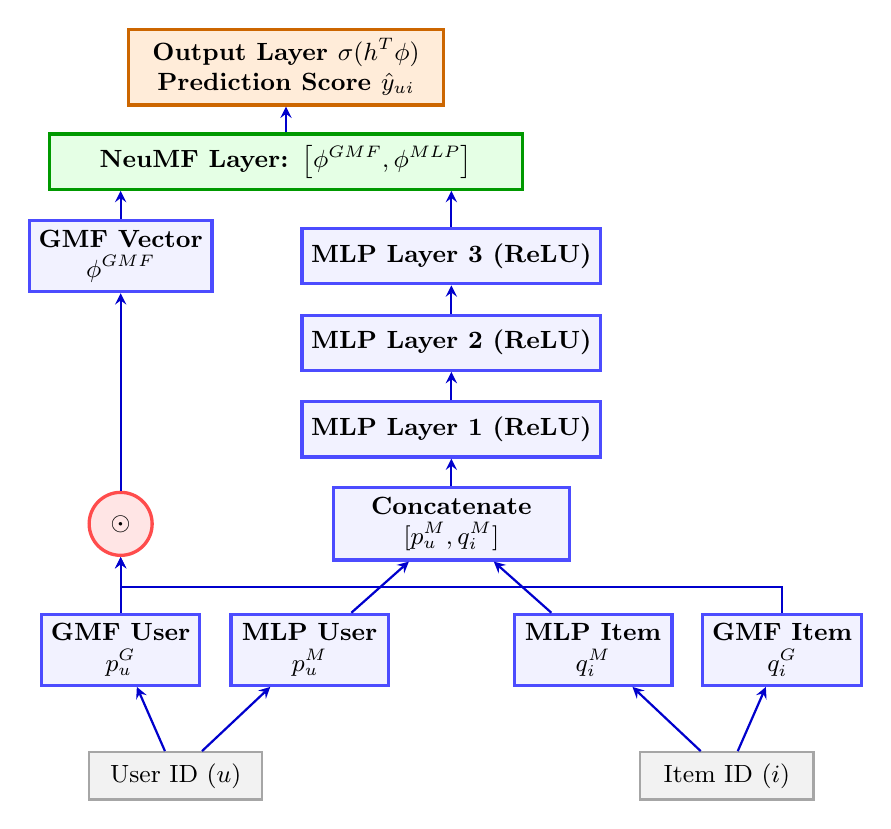
\begin{tikzpicture}[
        node distance=1.3cm,
        layer/.style={rectangle, draw=blue!70, fill=blue!5, very thick, minimum width=2.8cm, minimum height=0.7cm, font=\small\bfseries, align=center},
        op/.style={circle, draw=red!70, fill=red!10, very thick, minimum size=0.8cm, font=\small\bfseries},
        inputnode/.style={rectangle, draw=gray!70, fill=gray!10, thick, minimum width=2.2cm, minimum height=0.6cm, font=\small},
        arrow/.style={->, >=stealth, thick, color=blue!80!black}
    ]
        % Input IDs
        \node[inputnode] (user_id) at (-3.5, 0) {User ID ($u$)};
        \node[inputnode] (item_id) at (3.5, 0) {Item ID ($i$)};

        % Embeddings
        \node[layer, minimum width=2.0cm] (emb_ug) at (-4.2, 1.6) {GMF User\\$p_u^G$};
        \node[layer, minimum width=2.0cm] (emb_um) at (-1.8, 1.6) {MLP User\\$p_u^M$};
        \node[layer, minimum width=2.0cm] (emb_im) at (1.8, 1.6) {MLP Item\\$q_i^M$};
        \node[layer, minimum width=2.0cm] (emb_ig) at (4.2, 1.6) {GMF Item\\$q_i^G$};

        % Operations
        \node[op] (hadamard) at (-4.2, 3.2) {$\odot$};
        \node[layer, minimum width=3.0cm] (mlp_cat) at (0, 3.2) {Concatenate\\$[p_u^M, q_i^M]$};

        % MLP Hidden Layers
        \node[layer, minimum width=3.0cm] (mlp_1) at (0, 4.4) {MLP Layer 1 (ReLU)};
        \node[layer, minimum width=2.6cm] (mlp_2) at (0, 5.5) {MLP Layer 2 (ReLU)};
        \node[layer, minimum width=2.2cm] (mlp_3) at (0, 6.6) {MLP Layer 3 (ReLU)};

        % GMF Vector Node
        \node[layer, minimum width=2.0cm] (gmf_out) at (-4.2, 6.6) {GMF Vector\\$\phi^{GMF}$};

        % NeuMF Concat
        \node[layer, minimum width=6.0cm, fill=green!10, draw=green!60!black] (neumf_cat) at (-2.1, 7.8) {NeuMF Layer: $\left[ \phi^{GMF}, \phi^{MLP} \right]$};

        % Output
        \node[layer, minimum width=4.0cm, fill=orange!15, draw=orange!80!black] (output) at (-2.1, 9.0) {Output Layer $\sigma(h^T \phi)$\\Prediction Score $\hat{y}_{ui}$};

        % Connections
        \draw[arrow] (user_id) -- (emb_ug);
        \draw[arrow] (user_id) -- (emb_um);
        \draw[arrow] (item_id) -- (emb_im);
        \draw[arrow] (item_id) -- (emb_ig);

        \draw[arrow] (emb_ug) -- (hadamard);
        \draw[arrow] (emb_ig) -- ++(0, 0.8) -| (hadamard);

        \draw[arrow] (emb_um) -- (mlp_cat);
        \draw[arrow] (emb_im) -- (mlp_cat);

        \draw[arrow] (mlp_cat) -- (mlp_1);
        \draw[arrow] (mlp_1) -- (mlp_2);
        \draw[arrow] (mlp_2) -- (mlp_3);

        \draw[arrow] (hadamard) -- (gmf_out);

        \draw[arrow] (gmf_out) -- (neumf_cat.south -| gmf_out);
        \draw[arrow] (mlp_3) -- (neumf_cat.south -| mlp_3);

        \draw[arrow] (neumf_cat) -- (output);
    \end{tikzpicture}
    \caption{Sơ đồ kiến trúc chi tiết mô hình lai Neural Matrix Factorization (NeuMF)}
    \label{fig:neumf_architecture}
\end{figure}

\subsection{Chiến lược hợp nhất: Early Fusion và Late Fusion}
\label{subsec:early_late_fusion}

Khi một hệ gợi ý kết hợp nhiều nguồn thông tin hoặc nhiều góc nhìn (view) về người dùng và sản phẩm, có hai cách hợp nhất cơ bản, phân biệt theo \emph{mức} diễn ra phép hợp nhất \parencite{atrey2010multimodal, liu2018combine, holinh2023multisource}:

\begin{itemize}
    \item \textbf{Early Fusion (hợp nhất ở mức đặc trưng/biểu diễn):} các vector đặc trưng $v_1, \dots, v_m$ của từng view được nối thành một biểu diễn chung, rồi \emph{một} mô hình $h$ duy nhất học tương tác giữa chúng và đưa ra dự đoán:
    \begin{equation}
        p = h\big([v_1;\, v_2;\, \dots;\, v_m]\big)
        \label{eq:early_fusion}
    \end{equation}

    \item \textbf{Late Fusion (hợp nhất ở mức quyết định/điểm dự đoán):} mỗi view được xử lý bởi một mô hình riêng $h_j$ cho ra dự đoán độc lập, rồi các dự đoán được kết hợp bằng một cơ chế $F$ -- lấy trung bình, bỏ phiếu, trọng số cố định hoặc một mô hình học:
    \begin{equation}
        p = F\big(h_1(v_1),\, h_2(v_2),\, \dots,\, h_m(v_m)\big)
        \label{eq:late_fusion}
    \end{equation}
    Khi $F$ là tổng có trọng số, đây chính là kiểu lai \emph{weighted} trong phân loại hệ gợi ý lai của \textcite{burke2002hybrid}.
\end{itemize}
Ngoài hai cách trên còn có \emph{hybrid fusion}, kết hợp cả mức đặc trưng lẫn mức quyết định \parencite{atrey2010multimodal}. Early Fusion học được tương tác giữa các view nhưng đòi hỏi một mô hình phù hợp với mọi view; Late Fusion linh hoạt hơn nhưng không nắm bắt được tương tác ở mức tín hiệu giữa các view, vì chỉ làm việc trên kết quả dự đoán \parencite{holinh2023multisource}.

\textbf{Vị trí của các mô hình trong đề tài.} Hai view chính ở đây là hai cách mô hình hóa tương tác: view tuyến tính của nhánh MF (vector $p_u^G \odot q_i^G$ của GMF) và view phi tuyến của nhánh DNN (vector cuối $\phi_L^{MLP}$ của MLP). NeuMF nối hai vector này rồi đưa qua một lớp dự đoán chung (công thức~\eqref{eq:neumf_concat}--\eqref{eq:neumf_prediction}), nên là một mô hình \textbf{Early Fusion ở mức biểu diễn}, được huấn luyện chung từ đầu đến cuối (Hình~\ref{fig:fusion_compare}a). Mô hình đề tài NeuMF-F giữ nguyên cách hợp nhất này với hai nhánh có đặc trưng GMF-F và MLP-F; thêm vào đó, đặc trưng nội dung và ngữ cảnh được cộng vào vector của từng nhánh ngay ở đầu vào, tức cũng được hợp nhất sớm với thông tin cộng tác (mục~\ref{subsec:embedding_design}). Late Fusion tương ứng là trộn điểm của hai mô hình MF và DNN được huấn luyện \emph{riêng}:
\begin{equation}
    \hat{y}_{ui} = w\,\tilde{s}^{MF}_{ui} + (1-w)\,\tilde{s}^{DNN}_{ui}, \qquad
    \tilde{s}_{ui} = \frac{s_{ui} - \min_{j \in \mathcal{C}_u} s_{uj}}{\max_{j \in \mathcal{C}_u} s_{uj} - \min_{j \in \mathcal{C}_u} s_{uj}}
    \label{eq:late_fusion_mfdnn}
\end{equation}
trong đó điểm $s_{ui}$ của từng mô hình được chuẩn hóa min--max trên tập ứng viên $\mathcal{C}_u$ của User $u$ để hai thang điểm so sánh được, và $w \in [0, 1]$ được chọn trên tập xác thực ($w = 1$ và $w = 0$ cho đúng thứ hạng của từng thành phần). Để so sánh công bằng với NeuMF-F, đề tài dùng chính hai thành phần của nó -- \textbf{LateFusion-F} trộn điểm của GMF-F và MLP-F được huấn luyện riêng (Hình~\ref{fig:fusion_compare}b); so sánh hai cách hợp nhất này là một câu hỏi của họ kiểm định (mục~\ref{sec:protocol}). Riêng nhánh MLP khi đứng một mình chỉ nối vector User và Item ở đầu vào: đó là mô hình DNN thuần, không phải phép hợp nhất MF với DNN (mục~\ref{subsec:early_fusion_design}).

\begin{figure}[htbp]
    \centering
    \resizebox{\textwidth}{!}{%
    \begin{tikzpicture}[
        box/.style={rectangle, draw=blue!70, fill=blue!5, thick, rounded corners=2pt, minimum width=3.0cm, minimum height=0.8cm, font=\small, align=center},
        norm/.style={rectangle, draw=gray!70, fill=gray!8, thick, rounded corners=2pt, minimum width=2.6cm, minimum height=0.8cm, font=\small, align=center},
        fuse/.style={rectangle, draw=green!60!black, fill=green!10, thick, rounded corners=2pt, minimum width=3.6cm, minimum height=0.8cm, font=\small, align=center},
        outn/.style={rectangle, draw=orange!80!black, fill=orange!15, thick, rounded corners=2pt, minimum width=1.8cm, minimum height=0.7cm, font=\small},
        title/.style={font=\small\bfseries, align=center},
        arrow/.style={->, >=stealth, thick, color=blue!80!black}
    ]
        % (a) Early Fusion -- NeuMF
        \node[title] at (0, 5.9) {(a) Early Fusion -- NeuMF, NeuMF-F\\[1pt]\normalfont một mô hình, huấn luyện chung};
        \node[box] (ga) at (-1.8, 0) {Nhánh GMF (GMF-F)\\$\phi^{GMF} = p_u^G \odot q_i^G$};
        \node[box] (ma) at (1.8, 0) {Nhánh MLP (MLP-F)\\$\phi_L^{MLP}$};
        \node[fuse] (ca) at (0, 1.8) {Nối biểu diễn\\$[\phi^{GMF};\ \phi_L^{MLP}]$};
        \node[box, minimum width=3.6cm] (ha) at (0, 3.3) {Một lớp dự đoán chung\\$\sigma(h^T [\phi^{GMF};\ \phi_L^{MLP}])$};
        \node[outn] (ya) at (0, 4.75) {$\hat{y}_{ui}$};
        \draw[arrow] (ga) -- (ca);
        \draw[arrow] (ma) -- (ca);
        \draw[arrow] (ca) -- (ha);
        \draw[arrow] (ha) -- (ya);

        \draw[dashed, gray] (4.1, -0.7) -- (4.1, 6.4);

        % (b) Late Fusion GMF + MLP
        \node[title] at (8.2, 5.9) {(b) Late Fusion -- LateFusion-F\\[1pt]\normalfont hai mô hình huấn luyện riêng};
        \node[box] (gb) at (6.4, 0) {Mô hình GMF-F\\điểm $s^{GMF}_{ui}$};
        \node[box] (mb) at (10.0, 0) {Mô hình MLP-F\\điểm $s^{MLP}_{ui}$};
        \node[norm] (ngb) at (6.4, 1.8) {min--max trên $\mathcal{C}_u$\\$\tilde{s}^{GMF}_{ui}$};
        \node[norm] (nmb) at (10.0, 1.8) {min--max trên $\mathcal{C}_u$\\$\tilde{s}^{MLP}_{ui}$};
        \node[fuse] (fb) at (8.2, 3.3) {Trộn điểm ($w$ chọn trên tập xác thực)\\$w\,\tilde{s}^{GMF}_{ui} + (1-w)\,\tilde{s}^{MLP}_{ui}$};
        \node[outn] (yb) at (8.2, 4.75) {$\hat{y}_{ui}$};
        \draw[arrow] (gb) -- (ngb);
        \draw[arrow] (mb) -- (nmb);
        \draw[arrow] (ngb) -- (fb);
        \draw[arrow] (nmb) -- (fb);
        \draw[arrow] (fb) -- (yb);
    \end{tikzpicture}}
    \caption{Hai cách hợp nhất cùng hai thành phần MF (GMF) và DNN (MLP): ở mức biểu diễn (NeuMF, NeuMF-F) và ở mức điểm dự đoán (Late Fusion, LateFusion-F)}
    \label{fig:fusion_compare}
\end{figure}

\subsection{Lấy mẫu âm (Negative Sampling) và hàm tổn thất Binary Cross-Entropy}
\label{subsec:negative_sampling_loss}

Do dữ liệu phản hồi ẩn chỉ cung cấp các tương tác dương ($y_{ui} = 1$), kỹ thuật lấy mẫu âm (Negative Sampling) chọn ngẫu nhiên các Item mà User chưa từng tương tác để gán nhãn âm ($y_{ui} = 0$); đây là cách làm được He và cộng sự sử dụng khi huấn luyện NCF \parencite{he2017ncf}.

Hàm tổn thất Binary Cross-Entropy (BCE) được áp dụng để tối ưu hóa toàn bộ tham số mô hình:
\begin{equation}
    \mathcal{L}_{BCE} = -\sum_{(u, i) \in \mathcal{Y} \cup \mathcal{Y}^-} \left[ y_{ui} \log \hat{y}_{ui} + (1 - y_{ui}) \log (1 - \hat{y}_{ui}) \right]
    \label{eq:bce_loss}
\end{equation}
trong đó $\mathcal{Y}$ là tập tương tác dương và $\mathcal{Y}^-$ là tập cặp âm được lấy mẫu.

\section{Xu hướng nghiên cứu hiện đại trong hệ thống gợi ý học sâu}
\label{sec:modern_trends}

Sau NCF/NeuMF \parencite{he2017ncf}, lĩnh vực hệ gợi ý phát triển theo nhiều hướng song song. Mục này chỉ điểm qua những hướng liên quan trực tiếp tới vị trí của đề tài (mục~\ref{sec:khoangtrong_nghiencuu}) và tới các hướng phát triển (Chương~\ref{chap:ketluan}); các khảo sát của \textcite{zhang2019deeplearningsurvey} và \textcite{li2024dnncf} hệ thống hóa đầy đủ hơn.

\subsection{Mô hình lai dựa trên đặc trưng và khởi đầu lạnh của sản phẩm}
\label{subsec:deep_ctr}

Một nhánh phát triển trực tiếp của ý tưởng ``lai tuyến tính -- phi tuyến'' là các mô hình dùng nhiều đặc trưng hơn cặp mã User--Item, xuất phát từ bài toán dự đoán tỷ lệ nhấp chuột (Click-Through Rate -- CTR). Factorization Machines (FM) \parencite{rendle2010fm} tổng quát hóa MF cho vector đặc trưng bất kỳ: mỗi đặc trưng có một vector ẩn, và tương tác bậc hai giữa hai đặc trưng được mô hình hóa bằng tích vô hướng của hai vector ẩn đó; khi đặc trưng chỉ gồm mã User và mã Item, FM suy biến đúng về MF. Wide \& Deep \parencite{cheng2016wide} chạy song song một nhánh tuyến tính (Wide) để ghi nhớ các tổ hợp đặc trưng tường minh và một nhánh MLP (Deep) để khái quát hóa, hai nhánh được huấn luyện chung và cộng ở lớp đầu ra; DeepFM \parencite{guo2017deepfm} thay nhánh Wide bằng FM, hai nhánh dùng chung Embedding đặc trưng; Deep Interest Network \parencite{zhou2018din} thêm cơ chế Attention trên lịch sử hành vi. Điểm chung của các kiến trúc này -- một thành phần tuyến tính kiểu nhân tử hóa và một thành phần phi tuyến kiểu MLP, hợp nhất ở lớp dự đoán và huấn luyện chung -- chính là cấu trúc của NeuMF; khác biệt là đầu vào gồm cả đặc trưng chứ không chỉ mã ID. Mô hình đề tài NeuMF-F (mục~\ref{sec:model_design}) đi theo hướng này: giữ hai nhánh GMF và MLP của NeuMF, và biểu diễn mỗi User/Item bằng tổng của Embedding ID và một phép chiếu tuyến tính của đặc trưng.

Lợi ích quan trọng nhất của đặc trưng trên dữ liệu thời trang là xử lý \textbf{khởi đầu lạnh của sản phẩm}. Một sản phẩm mới chưa có tương tác nào nên không có Embedding ID có nghĩa, nhưng vẫn có thuộc tính và mô tả -- đủ để đặt nó gần những sản phẩm tương tự đã bán. \textcite{schein2002coldstart} chỉ ra rằng gợi ý cho đối tượng khởi đầu lạnh đòi hỏi kết hợp thông tin nội dung với dữ liệu cộng tác. DropoutNet \parencite{volkovs2017dropoutnet} đề xuất một kỹ thuật huấn luyện đơn giản cho mô hình nhận cả biểu diễn sở thích lẫn nội dung: khi huấn luyện, phần biểu diễn sở thích (học từ tương tác) của đối tượng bị bỏ ngẫu nhiên, buộc mô hình học cách chấm điểm chỉ từ nội dung -- đúng tình huống của đối tượng mới lúc dự đoán. NeuMF-F áp dụng ý tưởng này bằng cách bỏ ngẫu nhiên Embedding ID của sản phẩm khi huấn luyện (mục~\ref{subsec:embedding_design}).

Đặc trưng văn bản của sản phẩm (tên, mô tả) được biểu diễn theo cách cổ điển của truy hồi thông tin và lọc nội dung \parencite{lops2011content}: trọng số TF-IDF \parencite{salton1988term} -- từ xuất hiện nhiều trong mô tả của một sản phẩm nhưng hiếm trong toàn danh mục thì có trọng số cao -- rồi giảm chiều bằng phân rã giá trị kỳ dị rút gọn, tức phân tích ngữ nghĩa tiềm ẩn (Latent Semantic Analysis) \parencite{deerwester1990lsa}, để các mô tả dùng từ khác nhau nhưng cùng chủ đề có vector gần nhau. Cách biểu diễn này không cần dữ liệu tương tác và không cần tài nguyên tính toán lớn như các mô hình ngôn ngữ hiện đại.

\subsection{Gợi ý theo chuỗi hành vi và Transformer}
\label{subsec:sequential_rec}

NeuMF và MF coi lịch sử của User như một \emph{tập hợp không thứ tự}. Gợi ý theo chuỗi mô hình hóa trình tự $(i_1, \dots, i_t)$ để dự đoán $i_{t+1}$: GRU4Rec \parencite{hidasi2016gru4rec} dùng mạng hồi quy có cổng cho phiên duyệt web; SASRec \parencite{kang2018self} thay hồi quy bằng Self-Attention một chiều; BERT4Rec \parencite{sun2019bert4rec} dùng Transformer hai chiều, huấn luyện bằng cách che ngẫu nhiên một số vị trí trong chuỗi rồi dự đoán lại. Hướng này hợp với dữ liệu có phiên rõ ràng; trên H\&M, giao dịch chỉ ghi ngày mua (không có giờ hay mã phiên) và nhiều sản phẩm được mua cùng giỏ trong một ngày nên thứ tự trong ngày không xác định -- vì vậy đề tài dùng yếu tố thời gian để chia dữ liệu, để huấn luyện lại trên dữ liệu mới nhất (mục~\ref{subsec:split_sampling}) và làm đặc trưng tổng hợp (doanh số gần đây của sản phẩm, khoảng cách tới lần mua gần nhất của khách, mục~\ref{subsec:features}), còn mô hình chuỗi là hướng phát triển. Transformer còn được dùng theo cách khác: làm mô hình hợp nhất nhiều view theo kiểu Early Fusion, như trong hướng tích hợp đa nguồn của \textcite{holinh2023multisource}.

\subsection{Học biểu diễn trên đồ thị (Graph-based Collaborative Filtering)}
\label{subsec:graph_cf}

Ma trận tương tác User--Item có thể xem là một đồ thị hai phía. NGCF \parencite{wang2019ngcf} lan truyền Embedding qua láng giềng nhiều bước để vector mã hóa cả tín hiệu tương tác bậc cao (\textit{high-order connectivity}); LightGCN \parencite{he2020lightgcn} bỏ các phép biến đổi và hàm kích hoạt phi tuyến -- được chỉ ra là không cần thiết cho CF thuần -- và chỉ giữ phép lan truyền tuyến tính:
\begin{equation}
    e_u^{(k+1)} = \sum_{i \in \mathcal{N}_u} \frac{1}{\sqrt{|\mathcal{N}_u|}\sqrt{|\mathcal{N}_i|}} e_i^{(k)}, \qquad
    e_u^{*} = \sum_{k=0}^{K} \alpha_k \, e_u^{(k)}
    \label{eq:lightgcn}
\end{equation}
trong đó $\mathcal{N}_u$ là tập Item lân cận của User $u$ trên đồ thị và $e_u^{*}$ là biểu diễn cuối, tổng hợp có trọng số qua $K$ tầng lan truyền. LightGCN được báo cáo vượt MF và NGCF trên các bộ dữ liệu thưa như Gowalla và Amazon-Book \parencite{he2020lightgcn}; đây là một hướng phát triển của đề tài (mục~\ref{sec:huongphattrien}), với điều kiện được đánh giá theo cùng quy trình không thiên lệch.

\subsection{Mô hình tự mã hóa biến phân (Variational Autoencoder) cho lọc cộng tác}
\label{subsec:vae_cf}

Mult-VAE \parencite{liang2018multvae} nhận \emph{toàn bộ} vector mua $x_u \in \{0, 1\}^N$ của một User làm đầu vào, mã hóa thành một phân phối ẩn Gauss $q_\phi(z_u \mid x_u)$, rồi giải mã ra phân phối đa thức trên toàn bộ catalog $\pi(z_u) = \mathrm{softmax}(f_\theta(z_u))$. Mô hình được huấn luyện bằng cách cực đại cận dưới biến phân (ELBO), với hệ số $\beta$ điều chỉnh số hạng KL:
\begin{equation}
    \mathcal{L}_\beta(x_u) = \mathbb{E}_{q_\phi(z_u \mid x_u)}\big[\log p_\theta(x_u \mid z_u)\big] - \beta \cdot \mathrm{KL}\big(q_\phi(z_u \mid x_u)\,\big\|\,p(z_u)\big)
    \label{eq:multvae}
\end{equation}
với hàm hợp lý đa thức $\log p_\theta(x_u \mid z_u) = \sum_{i} x_{ui} \log \pi_i(z_u)$. Khác NeuMF (tính điểm từng cặp $(u, i)$ độc lập và cần lấy mẫu âm), Mult-VAE tính điểm cho cả catalog trong một lượt và dùng toàn bộ sản phẩm chưa mua làm tín hiệu âm, nên hợp tự nhiên với giao thức Full Ranking. Đề tài chưa cài đặt mô hình này; nó là một ứng viên cho nhánh học sâu ở hướng phát triển.

Các hướng mới hơn -- học tự giám sát trên đồ thị \parencite{wu2021sgl}, gợi ý sinh và mô hình ngôn ngữ lớn \parencite{rajput2023tiger, wu2023survey_llm4rec}, mô hình khuếch tán \parencite{wei2025diffusion} -- cần tài nguyên tính toán vượt phạm vi của đề tài (máy tính cá nhân), nên chỉ được ghi nhận ở đây. Ở quy mô công nghiệp, kiến trúc hai tháp \parencite{covington2016youtube} mã hóa User và Item thành hai vector độc lập để truy hồi bằng tìm kiếm lân cận gần đúng -- cũng là lý do mô hình tích vô hướng dễ triển khai hơn MLP khi catalog rất lớn. Khảo sát của \textcite{li2024dnncf} xác nhận các khối GMF/MLP theo tinh thần NCF vẫn được dùng phổ biến trong các hệ lai hiện đại, dù không còn là hướng tiên phong.

Trong phạm vi đề tài, kiến trúc hai nhánh của NeuMF -- bổ sung đặc trưng thành NeuMF-F -- được lựa chọn làm trọng tâm (thay vì các hướng mới hơn kể trên) vì ba lý do cụ thể: \textit{(i) Đặc điểm dữ liệu:} tệp giao dịch H\&M chỉ ghi ngày mua, không có phiên để áp dụng trực tiếp mô hình chuỗi (mục~\ref{subsec:sequential_rec}), nhưng có thuộc tính và mô tả văn bản của sản phẩm -- loại thông tin mà cách biểu diễn ``Embedding ID + đặc trưng'' khai thác được trực tiếp (mục~\ref{subsec:deep_ctr}); ảnh sản phẩm không được dùng vì chi phí tính toán; \textit{(ii) Mục tiêu khoa học:} kiến trúc hai nhánh GMF/MLP tách biệt cho phép bóc tách từng thành phần, so sánh trực tiếp hai cách hợp nhất trên cùng hai thành phần (mục~\ref{subsec:early_late_fusion}) và so sánh với chính NeuMF chỉ dùng ID để đo riêng đóng góp của đặc trưng -- điều khó làm tương đương với các kiến trúc End-to-End phức tạp hơn; \textit{(iii) Hạ tầng tính toán:} thực nghiệm chạy trên máy tính cá nhân với RAM 16 GB (mục~\ref{sec:exp_config}), không đủ cho các mô hình sinh quy mô lớn. Ba lý do này nhất quán với khoảng trống nghiên cứu ở mục~\ref{sec:khoangtrong_nghiencuu}.

\section{Các chỉ số đánh giá hệ thống gợi ý Top-K}
\label{sec:metrics}

Với mỗi người dùng được đánh giá $u$, mô hình xếp hạng tập ứng viên $\mathcal{C}_u$ và trả về danh sách $\text{Rec}_K(u)$ gồm $K$ sản phẩm đầu. Gọi $T_u$ là tập sản phẩm đúng của $u$ (với giao thức Leave-One-Out $|T_u| = 1$; với giao thức chia theo mốc thời gian chung của đề tài, một người dùng có thể có nhiều sản phẩm đúng) và $\text{hits}_u = |T_u \cap \text{Rec}_K(u)|$. Mọi chỉ số được tính cho từng người dùng rồi lấy trung bình trên tập người dùng được đánh giá $\mathcal{U}_{test}$.

\begin{itemize}
    \item \textbf{Hit Ratio at K (HR@K):} người dùng được tính là ``trúng'' nếu có ít nhất một sản phẩm đúng trong top-$K$ \parencite{he2017ncf}:
    \begin{equation}
        \text{HR@K} = \frac{1}{|\mathcal{U}_{test}|} \sum_{u \in \mathcal{U}_{test}} \mathbb{I}\left( \text{hits}_u \ge 1 \right)
        \label{eq:hr_k}
    \end{equation}

    \item \textbf{Precision@K và Recall@K:} tỉ lệ gợi ý đúng trong $K$ sản phẩm, và tỉ lệ sản phẩm đúng tìm lại được:
    \begin{equation}
        \text{Precision@K}(u) = \frac{\text{hits}_u}{K}, \qquad \text{Recall@K}(u) = \frac{\text{hits}_u}{|T_u|}
        \label{eq:precision_recall}
    \end{equation}
    Khi $|T_u| = 1$, Recall@K trùng HR@K và Precision@K $=$ HR@K$/K$ -- lý do các chỉ số này chỉ mang thông tin riêng khi người dùng có nhiều sản phẩm đúng.

    \item \textbf{Normalized Discounted Cumulative Gain at K (NDCG@K):} thưởng nhiều hơn khi sản phẩm đúng nằm ở vị trí cao, theo định nghĩa của Järvelin và Kekäläinen \parencite{jarvelin2002} với mức liên quan nhị phân:
    \begin{equation}
        \begin{aligned}
            \text{NDCG@K}(u) &= \frac{\text{DCG@K}(u)}{\text{IDCG@K}(u)}, \\
            \text{DCG@K}(u) &= \sum_{j=1}^{K} \frac{\mathbb{I}(\text{Rec}_K(u)_j \in T_u)}{\log_2(j + 1)}, \\
            \text{IDCG@K}(u) &= \sum_{j=1}^{\min(|T_u|, K)} \frac{1}{\log_2(j + 1)}
        \end{aligned}
        \label{eq:ndcg_k}
    \end{equation}
    IDCG là giá trị DCG khi mọi sản phẩm đúng xếp ở đầu danh sách, nên NDCG@K $\in [0, 1]$. Với $|T_u| = 1$ và sản phẩm đúng ở hạng $r$: NDCG@K $= 1/\log_2(r+1)$ nếu $r \le K$, ngược lại bằng 0.

    \item \textbf{Chỉ số theo nhóm sản phẩm đúng (cũ/mới):} để biết mô hình gợi ý đúng loại sản phẩm nào, tập sản phẩm đúng được tách thành $T^{cu}_u$ (sản phẩm đã có dữ liệu huấn luyện) và $T^{moi}_u$ (sản phẩm chưa từng bán trước mốc dự đoán, mục~\ref{subsec:split_sampling}). NDCG@K của nhóm được tính theo Công thức~\eqref{eq:ndcg_k} với $T_u$ thay bằng tập của nhóm, dùng \emph{cùng} danh sách xếp hạng đầy đủ -- tức sản phẩm đúng của nhóm kia được coi như không liên quan; người dùng không có sản phẩm đúng thuộc nhóm không được tính vào trung bình của nhóm.
\end{itemize}

\paragraph{Full Ranking và Sampled Ranking.} Một số công trình, trong đó có \textcite{he2017ncf}, đánh giá bằng cách xếp sản phẩm đúng giữa 100 ứng viên (1 đúng + 99 âm lấy mẫu) -- gọi là Sampled Ranking. \textcite{krichene2020sampled} chứng minh chỉ số trên tập ứng viên lấy mẫu không nhất quán với chỉ số trên toàn bộ catalog -- có thể đảo ngược kết luận ``A tốt hơn B'' -- và khuyến nghị tránh lấy mẫu. Đề tài vì vậy chỉ dùng \textbf{Full Ranking}: xếp hạng toàn bộ tập ứng viên (khoảng 17 nghìn sản phẩm, gồm cả sản phẩm mới) trừ sản phẩm người dùng đã mua. Một phép đối chiếu với Sampled-99 ở giai đoạn phát triển cho thấy thứ hạng giữa các mô hình thay đổi giữa hai giao thức (mục~\ref{sec:v1_history}).

\subsection{Các chỉ số đánh giá ngoài độ chính xác (Beyond-Accuracy Metrics)}
\label{subsec:beyond_accuracy}

Chỉ tối ưu HR@K/NDCG@K có thể khiến mô hình thiên lệch về việc luôn gợi ý các sản phẩm phổ biến nhất (\textit{popularity bias}), vốn dễ trúng nhưng ít giá trị cá nhân hóa \parencite{vargas2011novelty}. Để mô tả danh sách gợi ý ngoài độ chính xác, đề tài dùng hai chỉ số:
\begin{itemize}
    \item \textbf{Độ phủ (Coverage):} tỉ lệ sản phẩm của không gian ứng viên $\mathcal{I}_{cand}$ xuất hiện trong danh sách gợi ý của ít nhất một người dùng:
    \begin{equation}
        \text{Coverage@K} = \frac{\left| \bigcup_{u \in \mathcal{U}_{test}} \text{Rec}_K(u) \right|}{|\mathcal{I}_{cand}|}
        \label{eq:coverage}
    \end{equation}
    Độ phủ thấp cho thấy mô hình chỉ khai thác một phần nhỏ danh mục -- trường hợp giới hạn là Most Popular, mọi người dùng nhận gần như cùng một danh sách.
    \item \textbf{Tỉ lệ sản phẩm mới trong danh sách gợi ý:} trung bình theo người dùng của tỉ lệ sản phẩm mới (chưa từng bán trước mốc dự đoán) trong top-$K$. Mô hình chỉ dùng ID luôn có tỉ lệ này bằng 0; với mô hình có đặc trưng, chỉ số cho biết mô hình có thực sự đưa sản phẩm mới vào gợi ý hay không.
\end{itemize}
Hai chỉ số này chỉ mang tính mô tả và được trình bày cạnh NDCG@K trong Chương~\ref{chap:thucnghiem}.

\section{Tổng quan các công trình nghiên cứu liên quan}
\label{sec:related_work}

Bảng~\ref{tab:related_work} tổng hợp các công trình nền tảng liên quan trực tiếp đến hướng tiếp cận của dự án.

\begin{xltabular}{\textwidth}{|p{3.2cm}|p{2.8cm}|p{2.5cm}|X|}
    \caption{Tổng quan các công trình nghiên cứu liên quan}
    \label{tab:related_work} \\
    \hline
    \textbf{Tác giả \& Năm} & \textbf{Mô hình / Phương pháp} & \textbf{Dữ liệu} & \textbf{Đóng góp chính \& Hạn chế} \\
    \hline
    \endfirsthead
    \hline
    \textbf{Tác giả \& Năm} & \textbf{Mô hình / Phương pháp} & \textbf{Dữ liệu} & \textbf{Đóng góp chính \& Hạn chế} \\
    \hline
    \endhead
    \hline
    \endfoot
    \textbf{Sarwar et al. (2001)} \cite{sarwar2001item} & Item-based CF (ItemKNN) & MovieLens & Gợi ý theo độ tương đồng giữa sản phẩm, tính trước được và dễ diễn giải. \textit{Hạn chế:} ma trận tương đồng tăng bậc hai theo số sản phẩm; chất lượng giảm khi dữ liệu quá thưa. \\
    \hline
    \textbf{Rendle et al. (2009)} \cite{rendle2009bpr} & BPR (Bayesian Personalized Ranking) & MovieLens, Netflix & Khung tối ưu dựa trên so sánh cặp cho implicit feedback. \textit{Hạn chế:} mô hình tuyến tính. \\
    \hline
    \textbf{He et al. (2017)} \cite{he2017ncf} & NCF / NeuMF & MovieLens, Pinterest & Đề xuất khung NCF kết hợp GMF và MLP; báo cáo NeuMF tốt hơn các baseline trên hai bộ dữ liệu của bài. \textit{Hạn chế:} chưa tích hợp đặc trưng nội dung. \\
    \hline
    \textbf{Cheng et al. (2016)} \cite{cheng2016wide} & Wide \& Deep Learning & Google Play Store & Kết hợp ghi nhớ (Wide) và khái quát hóa (Deep). \textit{Hạn chế:} cần kỹ nghệ đặc trưng thủ công. \\
    \hline
    \textbf{Guo et al. (2017)} \cite{guo2017deepfm} & DeepFM & Criteo, Dữ liệu doanh nghiệp & Thay Wide bằng Factorization Machine. \textit{Hạn chế:} chi phí tính toán tăng khi số đặc trưng lớn. \\
    \hline
    \textbf{Volkovs et al. (2017)} \cite{volkovs2017dropoutnet} & DropoutNet & CiteULike, RecSys Challenge 2017 & Huấn luyện mô hình nhận cả biểu diễn sở thích và nội dung, bỏ ngẫu nhiên phần sở thích để mô hình chấm được đối tượng khởi đầu lạnh. \textit{Hạn chế:} cần đặc trưng nội dung đủ giàu thông tin. \\
    \hline
    \textbf{Kang \& McAuley (2018)} \cite{kang2018self} & SASRec (Self-Attention tuần tự) & Amazon, Steam, MovieLens & Mô hình hóa chuỗi hành vi bằng Self-Attention. \textit{Hạn chế:} cần mốc thời gian/phiên rõ ràng, chưa khai thác được với dữ liệu chỉ ghi ngày mua như H\&M. \\
    \hline
    \textbf{Wang et al. (2019); He et al. (2020)} \cite{wang2019ngcf, he2020lightgcn} & NGCF / LightGCN (Graph-based CF) & Gowalla, Amazon-Book, Yelp2018 & Lan truyền tín hiệu tương tác bậc cao qua đồ thị hai phía. \textit{Hạn chế:} chi phí tính toán lan truyền tăng theo số tầng, chi phí tăng nhanh theo quy mô đồ thị khi catalog lớn. \\
    \hline
    \textbf{Li et al. (2024)} \cite{li2024dnncf} & Khảo sát DNN cho Collaborative Filtering & Tổng hợp đa miền (2020--2024) & Hệ thống hóa các kiến trúc MLP, CNN, RNN, GNN, Autoencoder, GAN đã tích hợp vào CF, xác nhận GMF/MLP vẫn là thành phần nền tảng phổ biến. \textit{Hạn chế:} khảo sát tổng hợp, không đề xuất mô hình mới hay thực nghiệm riêng. \\
    \hline
    \textbf{Liang et al. (2018)} \cite{liang2018multvae} & Mult-VAE (tự mã hóa biến phân) & MovieLens-20M, Netflix, Million Song & Mô hình hóa cả vector mua của User bằng phân phối đa thức, chấm toàn bộ catalog trong một lượt. \textit{Hạn chế:} không dùng thứ tự thời gian; cần đủ lịch sử cho mỗi User. \\
    \hline
    \textbf{Hồ Thị Linh (2023)} \cite{holinh2023multisource} & Tích hợp đa nguồn: Late Fusion (bỏ phiếu, MLP) và Early Fusion Utility Matrix + văn bản (TF-IDF, BERT), Transformer & MovieLens, Amazon & Hệ thống hóa Early/Late Fusion cho hệ gợi ý đa nguồn; Transformer hợp nhất nhiều view cải thiện độ chính xác dự đoán rating. \textit{Khác với đề tài:} bài toán dự đoán rating (MAE/RMSE) có nguồn văn bản; đề tài áp dụng phân loại Early/Late Fusion cho xếp hạng Top-K trên phản hồi ẩn. \\
    \hline
    \textbf{Ferrari Dacrema et al. (2019)} \cite{dacrema2019progress} & Tái lập 18 mô hình gợi ý học sâu & MovieLens, Pinterest, Netflix, \ldots & Phần lớn mô hình học sâu được tái lập không vượt baseline đơn giản được tinh chỉnh tốt (ItemKNN, SLIM); chỉ ra mã nguồn NCF chọn số epoch trên tập kiểm thử. \textit{Hạn chế:} chủ yếu dùng giao thức lấy mẫu của các bài gốc. \\
    \hline
    \textbf{Rendle et al. (2020)} \cite{rendle2020ncfmf} & MF tích vô hướng so với NeuMF & MovieLens 1M, Pinterest & MF được tinh chỉnh kỹ vượt NeuMF trên chính dữ liệu và giao thức của bài NCF; MLP khó học được tích vô hướng và không phù hợp truy hồi nhanh. \textit{Hạn chế:} vẫn dùng giao thức Leave-One-Out lấy mẫu của bài gốc. \\
    \hline
    \textbf{Dự án đề xuất (2026)} & NeuMF-F: hai nhánh GMF-F, MLP-F (Embedding ID + đặc trưng sản phẩm, khách hàng, thời gian), hợp nhất sớm & H\&M Personalized Fashion Recommendations (hai mẫu khách hàng độc lập) & Tập ứng viên gồm cả sản phẩm mới, đặc trưng theo thời điểm; tinh chỉnh trên mẫu phát triển, đánh giá một lần trên mẫu khách hàng độc lập theo kế hoạch đăng ký trước, 5 seed, kiểm định cặp có hiệu chỉnh Holm; so với NeuMF chỉ dùng ID, từng nhánh, Late Fusion của cùng hai nhánh và sáu baseline được tinh chỉnh cùng ngân sách; ablation từng nhóm đặc trưng. \\
    \hline
\end{xltabular}

Các công trình trong Bảng~\ref{tab:related_work} dùng dữ liệu, cách chia dữ liệu và giao thức đánh giá khác nhau; bảng chỉ tổng hợp phương pháp và đóng góp để làm cơ sở lựa chọn cách làm cho đề tài, không dùng số liệu của các công trình này làm chuẩn so sánh với kết quả của đề tài.

\section{Khoảng trống nghiên cứu}
\label{sec:khoangtrong_nghiencuu}

Các nghiên cứu nền tảng về NCF/NeuMF \parencite{he2017ncf} chủ yếu được đánh giá trên dữ liệu điện ảnh (MovieLens) hoặc mạng xã hội hình ảnh (Pinterest), với tín hiệu tương tác nhị phân và giao thức Leave-One-Out; tập sản phẩm của những bộ dữ liệu này gần như cố định, nên giới hạn khởi đầu lạnh của sản phẩm ít được đo. Các tái đánh giá về sau \parencite{dacrema2019progress, rendle2020ncfmf} cho thấy NeuMF chỉ dùng ID khó vượt các baseline đơn giản được tinh chỉnh kỹ. Các mô hình dùng đặc trưng (mục~\ref{subsec:deep_ctr}) giải quyết được khởi đầu lạnh, nhưng thường được đánh giá cho bài toán dự đoán nhấp chuột chứ không phải xếp hạng Top-K trên toàn bộ danh mục. Còn các hướng mới hơn như Graph-based CF \parencite{wang2019ngcf, he2020lightgcn}, Sequential Recommendation \parencite{kang2018self, sun2019bert4rec} hay LLM-based Recommendation \parencite{wu2023survey_llm4rec, rajput2023tiger} đòi hỏi cấu trúc dữ liệu đặc thù hoặc tài nguyên tính toán vượt phạm vi của đề tài.

Khoảng trống mà đề tài tập trung giải quyết vì vậy là: xây dựng một mô hình lai giữ cấu trúc MF + DNN của NeuMF nhưng khai thác được đặc trưng sản phẩm, khách hàng và thời gian (NeuMF-F), rồi đánh giá nó trên dữ liệu giao dịch thời trang thực tế (H\&M) theo một giao thức gần với tình huống triển khai -- sản phẩm mới nằm trong tập ứng viên, đặc trưng không dùng thông tin tương lai, kết luận lấy trên một mẫu khách hàng chưa từng được dùng để ra quyết định -- và tránh các lỗi phương pháp mà \textcite{dacrema2019progress} và \textcite{rendle2020ncfmf} đã chỉ ra (chọn mô hình trên tập kiểm thử, baseline tinh chỉnh sơ sài, chỉ số trên tập ứng viên lấy mẫu). Thiết kế đối chứng cho phép tách riêng ba câu hỏi: đặc trưng có giúp mô hình lai không (NeuMF-F so với NeuMF), hợp nhất có giúp so với từng nhánh không (NeuMF-F so với GMF-F, MLP-F), và hợp nhất sớm hay hợp nhất muộn phù hợp hơn (NeuMF-F so với LateFusion-F, theo phân loại của \textcite{holinh2023multisource}).